\newpage

\onecolumn

\appendix

\section{Messwerte}
\label{sec:messwerte}
OO-Messwerte

auch die ausm laborbuch!!!

\begin{figure}[htb!]
 \centering
 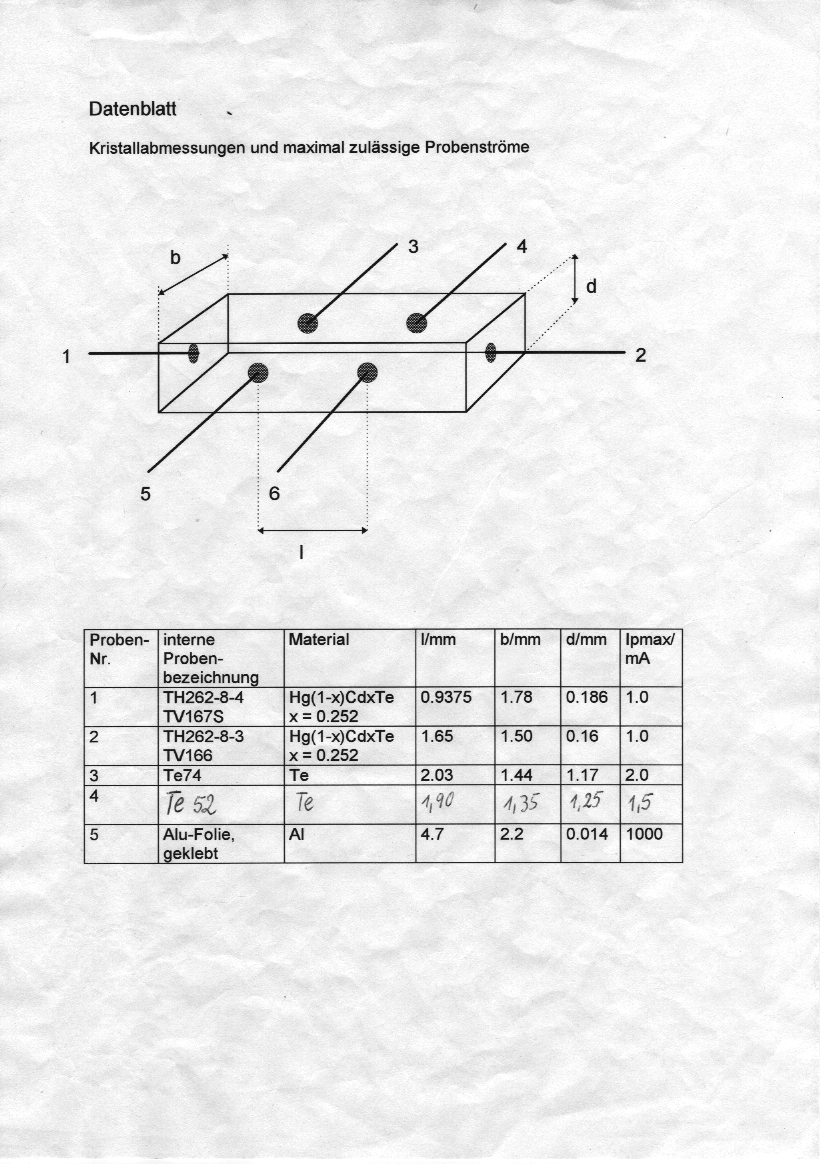
\includegraphics[viewport=40 420 470 700,clip]{../docs/scan_datenblatt}
 % scan_datenblatt.png: 824x1164 pixel, 100dpi, 20.93x29.57 cm, bb=0 0 593 838
 \caption{Abmessungen}
 \label{fig:abmessungen}
\end{figure}



\begin{table}[htb!]
 \centering
 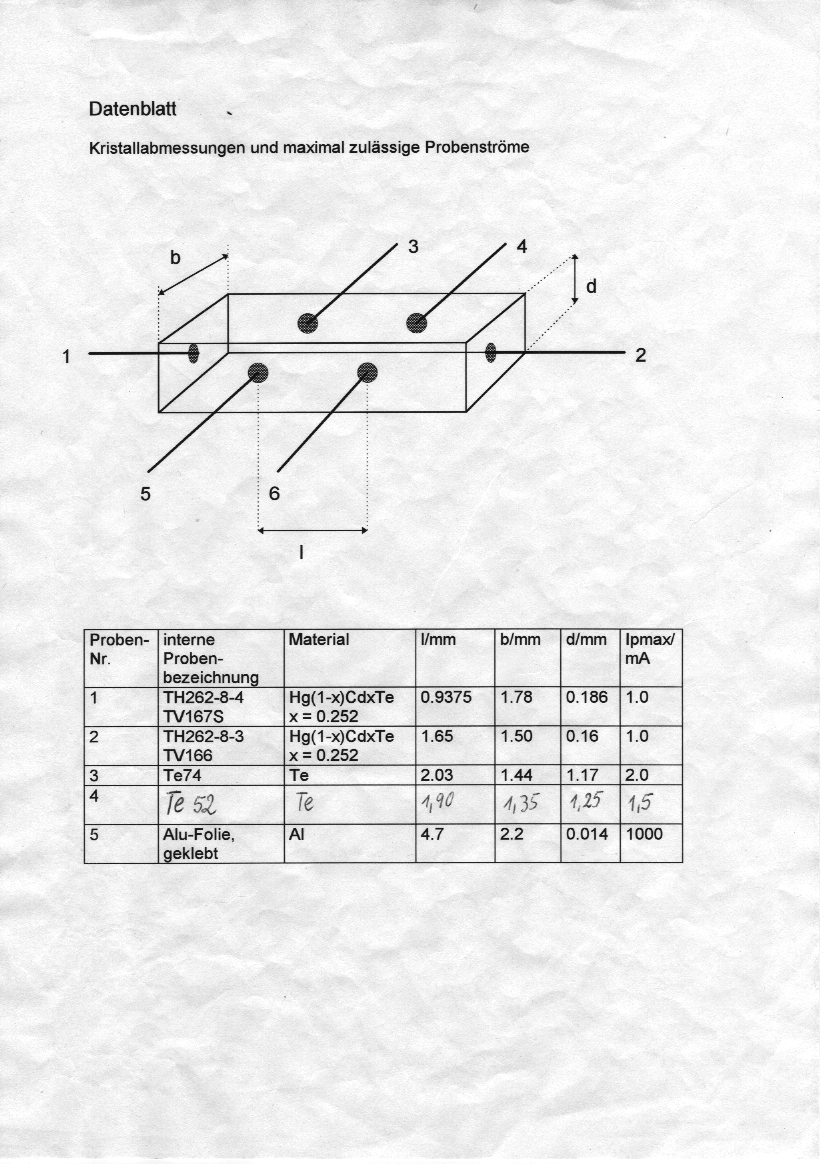
\includegraphics[viewport=55 200 500 390,clip]{../docs/scan_datenblatt}
 % scan_datenblatt.png: 824x1164 pixel, 100dpi, 20.93x29.57 cm, bb=0 0 593 838
 \caption{Daten}
 \label{tab:daten}
\end{table}